\documentclass{article}
\usepackage{graphicx}
\usepackage[margin=1.5cm]{geometry}
\usepackage{amsmath}

\begin{document}
\twocolumn

\title{Warm Up: Energy I}
\author{Prof. Jordan C. Hanson}

\maketitle

\section{Memory Bank}

\begin{itemize}
\item $W = \vec{F} \cdot \Delta \vec{x}$ ... Definition of work (1 N m, or 1 Joule)
\item $\vec{F} = -k\Delta \vec{x}$ ... Hooke's Law, or the force of a spring
\item $\vec{f} = -\mu N \hat{i}$ ... Force of friction on a flat surface
\item $KE = \frac{1}{2}m v^2$ ... Definition of Kinetic Energy
\item $W = KE_f - KE_i$ ... Work-energy theorem
\item Gravitational potential energy: $U = mgh$, where $h$ is the height, $m$ is the mass, and $g$ is the gravitational constant.
\end{itemize}

\section{Work and Energy}

\begin{enumerate}
\item Suppose a force $\vec{F} = 20\hat{i} - 20\hat{j}$ N acts on a mass, and displaces it by $\Delta \vec{x} = 0.4\hat{i} - 0.4\hat{j}$ m.  (a) What is the work done?  (b) What is the change in kinetic energy? (c) If the mass is 40 kg, what is the final velocity after the given displacement is reached? (d) Repeat the calculations for $\Delta \vec{x} = -0.4\hat{j}$ m. \\ \vspace{4.5cm}
\item Suppose we use a rope to lift a 25 kg object 10 meters above the ground.  (a) How much work does this require? (b) What is the gravitational potential energy? (b) What is the speed if it is dropped to the ground? \\ \vspace{3cm}
\item In the previous problem, what happens to the final speed if the height is doubled? \\ \vspace{1cm}
\item Consider Fig. \ref{fig:1}. A crate of mass 200 kg is to be brought from a site on the ground floor (A) to a third floor apartment (E). The workers know that they can either use the elevator first, then slide it along the third floor to the apartment, or first slide the crate to another location marked C below, and then take the elevator to the third floor and slide it on the third floor a shorter distance. The coefficient of kinetic friction between the crate and the ground floor is 0.100 and between the crate and the third floor is 0.300.  Find the work needed by the workers for each path shown from A to E. Assume that the force the workers need to do is just enough to slide the crate at constant velocity (zero acceleration).  The work by the elevator against the force of gravity is not done by the workers. 
\end{enumerate}

\begin{figure}
\centering
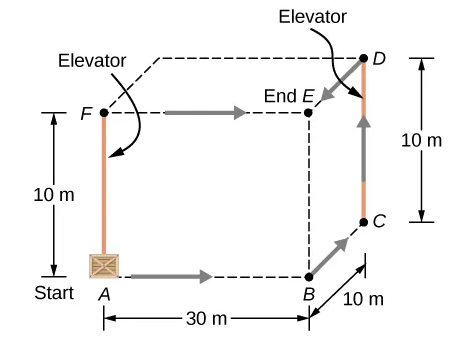
\includegraphics[width=0.5\textwidth]{figures/elevator.png}
\caption{\label{fig:1} Building diagram, with paths from point A to E.}
\end{figure}

\end{document}
